\documentclass{standalone}
\usepackage{tikz}
\usepackage{amsmath}

\begin{document}

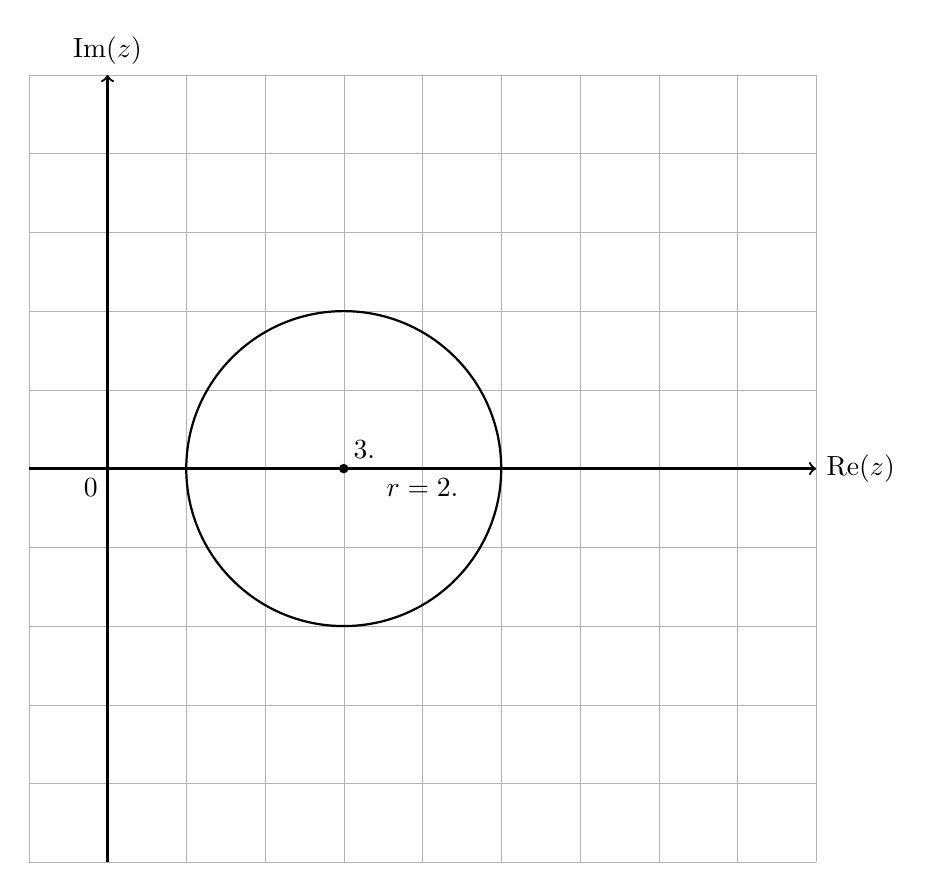
\begin{tikzpicture}
    
    % Center of the circle
    \def\xmin{-1}
    \def\xmax{9}
    \def\ymin{-5}
    \def\ymax{5}
    \def\dx{.5}
    \def\dy{.5}
    \def\xminb{\xmin-\dx}
    \def\xmaxb{\xmax+\dx}
    \def\yminb{\ymin-\dy}
    \def\ymaxb{\ymax+\dy}
    \coordinate (center) at (3., 0.);
    \def\radius{2.}

    % Draw grid
    \draw[step=1., gray!60, ultra thin] (\xmin, \ymin) grid (\xmax, \ymax); % Visible grid with lighter color
    
    % Axes
    \draw[->, thick] (\xmin, 0) -- (\xmax, 0) node[right] {$\text{Re}(z)$};
    \draw[->, thick] (0, \ymin) -- (0, \ymax) node[above] {$\text{Im}(z)$};

%   % Axis ticks
%   \foreach \x in {\xmin,..., \xmax}
%       \draw (\x, -0.1) -- (\x, 0.1) node[below=8pt] {\small $\x$};
%   \foreach \y in {\ymin,..., \ymax}
%       \draw (-0.1, \y) -- (0.1, \y) node[left=8pt] {\small $\y$};

    % Labels for axes
    \node[below left] at (0, 0) {$0$};

    % Circle
    \draw[thick] (center) circle (\radius);
    
    % Center point
    \filldraw[black] (center) circle (1.5pt) node[above right] {$3.$};
    
    % Radius line
    \draw[dashed] (center) -- ++(2, 0) node[midway, below] {$r = \radius$};
%   % Parametric equations x(t) = 2 + t, y(t) = 3 + 2t
%   \draw[thick,->] (-1, -3) -- (5, 9); % Just for reference
%   \draw[thick, blue] plot[parametric, domain=-3:3] 
%       (2 + \x, {3 + 2*\x}); % Draw the parametric line
        
\end{tikzpicture}

\end{document}
